\subsection{Definicja}
\begin{definition}
    Mówimy, że zmienna losowa \( X \) ma \textbf{rozkład jednostajny} na przedziale \( \brackets{a, b} \) jeśli dystrybuanta tej zmiennej zadana jest przez funkcję
    \[
        F(x) = \begin{cases}
            0 & \text{ gdy } x < a \\
            \frac{x - a}{b - a} & \text{ gdy } a \leq x \leq b \\
            1 & \text{ gdy } x > b
        \end{cases}
    \]
\end{definition}
Łatwo zauważyć, że gęstość takiej zmiennej wynosi \( \frac{1}{b-a} \) w \( \brackets{a, b} \) oraz 0 wszędzie indziej.

\begin{theorem}
    Niech \( X \) ma rozkład jednostajny na przedziale \( \brackets{a, b} \). Wtedy
    \[
        \expected{X} = \frac{a + b}{2}
    \]
\end{theorem}

\begin{theorem}
    Niech \( X \) ma rozkład jednostajny na przedziale \( \brackets{a, b} \). Wtedy
    \[
        \variance{X} = \frac{(b-a)^2}{12}
    \]
\end{theorem}


\begin{theorem}
    Niech \( X \) ma rozkład jednostajny na przedziale \( \brackets{a, b} \). Wtedy
    \[
        M_X(t) = \begin{cases}
            \frac{e^{tb} - e^{ta}}{t(b-a)} & \text{ dla } t \neq 0 \\
            1 \text{ dla } t = 0
        \end{cases}
    \]
\end{theorem}

\begin{theorem}
    Niech \( X \) ma rozkład jednostajny na przedziale \( \brackets{a, b} \). Wtedy dla dowolnych \( a \leq c \leq d \leq b \)
    \[
        P(X \leq c \mid X \leq d) = \frac{c - a}{d - a}
    \]
\end{theorem}
\begin{proof}
    \begin{align*}
        \frac{P\left( X\le c \cap X\le d  \right) }{P\left( X\le d  \right) } = \frac{P\left( X\le c  \right) }{P\left( X\le d  \right) } = \frac{c-a}{b-a} \cdot \frac{b-a}{d-a} = \frac{c-a}{d-a}.
    \end{align*}
\end{proof}


\begin{theorem}
    Niech \( X_1, \dots, X_n \) będą niezależne i wszystkie mają rozkład jednostajny na \( \brackets{0, 1} \).
    Ponadto, niech \( Y_1, \dots, Y_n \) będą tymi samymi wartościami, posortowanymi rosnąco. Wtedy
    \[
        \expected{Y_k} = \frac{k}{n + 1}
    \]
\end{theorem}
\begin{proof}
    Modyfikujemy lekko problem i zamiast wybierać \( n \) punktów z odcinka będziemy wybierać \( n + 1 \) punktów z łuku \(P_0, \dots, P_n\).
    W ten sposób \( X_i \) jest odległością zgodnie ze wskazówkami zegara punktów \( P_0, P_i \), 
    natomiast \( Y_k \) jest odległością od \( P_0 \) do \(k\)-tego punktu zgodnie ze wskazówkami zegara.
    
    Mamy \( n + 1 \) łuków między punktami i, ze względu na symetrię, oczekiwana długość łuku między dwoma sąsiednimi punktami wynosi \( \frac{1}{n + 1} \).
    
    W takim razie oczekiwana wartość \( Y_k \) to oczekiwana łączna długość \( k \) sąsiednich łuków, która wynosi \( \frac{k}{n + 1} \).
\end{proof}

\newpage
\subsection{Ćwiczenia}
\begin{exercise}
    \label{breaking-sticks-in-three-parts}
    Łamiemy kij długości jednego metra w dwóch miejscach wybranych niezależnie i jednostajnie.
    
    Podaj oczekiwaną długość najkrótszego, średniego, i najdłuższego kawałka.
\end{exercise}

\begin{proof}
Niech \(X\) i \(Y\) oznaczają odległości punktów podziału odpowiednio od lewego i prawego końca.

Jeśli \(X + Y \geq 1\) to znaczy, że punkty \(X, Y\) są zamienione kolejnością tj. \(Y\) jest bliżej lewego końca a \(X\) prawego.

Wygodniej nam będzie jednak gdy \(X + Y \leq 1\) więc zanim przejdziemy do głównej części pokażmy mini-lemat

Niech \(A\) będzie dowolną zmienną losową.

Ponieważ \(P(X \leq Y) = P(X + Y \leq 1) = \frac{1}{2} \) to 
\[
    \expected{A} =
        \expected{A \mid X \leq Y} \cdot P(X + Y \leq 1) + 
        \expected{A \mid X \geq Y} \cdot P(X + Y \geq 1)
\]

Zatem
\[
    \expected{A} = \frac{1}{2} \cdot \pars{\expected{A \mid X + Y \leq 1} + \expected{A \mid X + Y \geq 1}}
\]
Jeśli wartości przyjmowane przez \(A\) są symetryczne (a w naszym przypadku będą)
to \( \expected{A} = \expected{A \mid X + Y \leq 1} \).


Widzimy, że długości kawałków są niezależne od kolejności punktów a jedynie od ich pozycji, 
zatem możemy założyć, że \(X + Y \leq 1\)
Skoro \(X + Y \leq 1\) to punkty te dzielą kij na kawałki o długościach \(X, Y, 1 - X - Y\)


Niech \(A = \min(X, Y, 1 - X - Y), B = \text{mid}(X, Y, 1 - X - Y), C = \max(X, Y, 1 - X - Y)\)
Z liniowości wartości oczekiwanej mamy \(\expected{A} + \expected{B} + \expected{C} = \expected{A + B + C} = 1\),
wystarczy zatem policzyć \(\expected{A}\) oraz \(\expected{C}\).

Aby policzyć \(\expected{A}\)będziemy chcieli skorzystać z lematu \ref{continuous-positive-random-variable-lemma}.

Zacznijmy więc od policzenia \( P(A \geq a) \) dla dowolnego \(a \in \real\)

Widzimy, że \( P(A \geq a) = P(X \geq a \land Y \geq a \land 1 - X - Y \geq a) \)
Możemy zobrazować te zależności geometrycznie:

\begin{figure}[H]
    \centering
    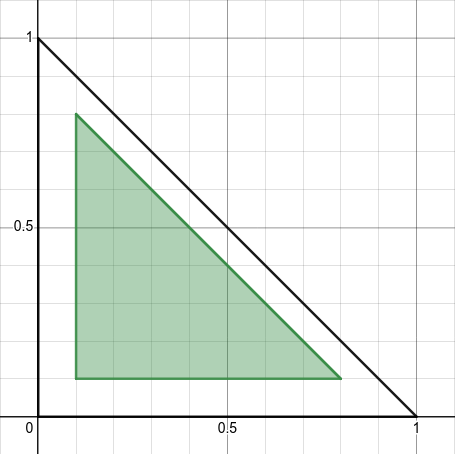
\includegraphics[scale=0.5]{img/continuous probability/breaking-stick-minimum-area.png}
    \caption{Obszar w którym zachodzą nierówności dla \(a = 0.1\)}
\end{figure}

Możemy policzyć pole tego trójkąta -- wynosi ono dokładnie \( \frac{(1 - 3a)^2}{2} \)
Pole dużego trójkąta wynosi \(\frac{1}{2}\) zatem \( P(A \geq a) = (1 - 3a)^2 = 9a^2 - 6a + 1 \)

Widzimy tutaj, że sens ma jedynie rozważanie \(a \leq \frac{1}{3} \) zatem finalnie

\[
    \expected{A} = \int_0^{\frac{1}{3}} P(A \geq a) \diff a
    = \int_0^{\frac{1}{3}} (9a^2 - 6a + 1) \diff a = \frac{1}{9}
\]

Policzenie \(\expected{C}\) jest bardzo podobne -- zamiast brać koniunkcji trzech warunków
to bierzemy ich alternatywę i liczymy pola otrzymanych figur. Pozostawiamy to jako ćwiczenie dla Czytelnika

\textit{Hint: Rozważ przedziały \( a \in \pars{0, \frac{1}{3}}, a \in \pars{\frac{1}{3}, \frac{1}{2}}, a \in \pars{\frac{1}{2}, 1} \). Poprawny wynik to \(\frac{11}{18}\)}
\end{proof}
\newpage
\begin{exercise}
    Losujemy \( X \) oraz \( Y \) niezależnie i jednostajnie z przedziału \( \brackets{0, 10} \).
    Jakie jest prawdopodobieństwo, że \( |X - Y| < 5 \) ? 
\end{exercise}
\begin{proof}
    Podobnie jak w ćwiczeniu \ref{breaking-sticks-in-three-parts} będziemy się warunkować pod założeniem, że \( X < Y \) argumentując tym, że wartość bezwzględna jest symetryczna.
    
    \begin{figure}[H]
        \centering
        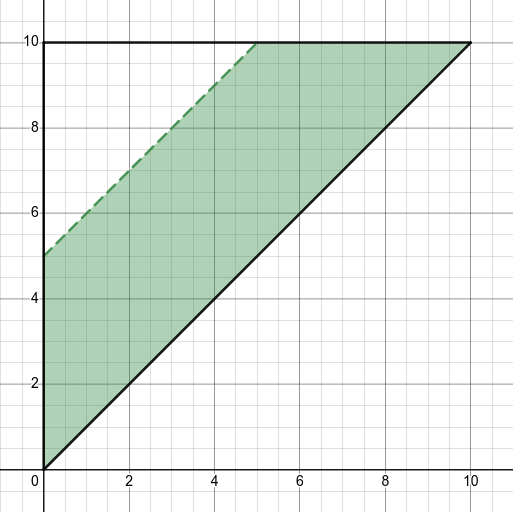
\includegraphics[scale=0.5]{img/continuous probability/distance-of-two-uniform-variables.png}
        \caption{Obszar w którym \( |X - Y| < 5\) }
    \end{figure}
    
    Widać, że dopełnienie tego zdarzenia jest trójkątem o boku 5, a całość jest trójkątem o boku 10,
    zatem \( P(|X - Y| \geq 5) = \frac{1}{4} \), czyli \( P(|X - Y| < 5) = \frac{3}{4} \)
\end{proof}
